\documentclass{fmbvecto}

\usepackage[spanish]{babel}

\renewcommand{\title}{Ejemplo de resolución correcta del Taller 1}
\newcommand{\subject}{Cálculo Vectorial}

\renewcommand{\labelenumii}{\theenumii}
\renewcommand{\theenumii}{\theenumi.\arabic{enumii}.}

\NewDocumentCommand{\itemp}{o}{\item (#1 puntos)}

\begin{document}

Domingo, 23 de junio de 2024

\begin{center}
    \textbf{\LARGE \title} \\
    {\large \subject}
\end{center}

Profesor: Jacinto Eloy Puig Portal, \href{mailto:jpuig@uniandes.edu.co}{jpuig@uniandes.edu.co}. \\
Monitor: Federico Melo Barrero, \href{mailto:f.melo@uniandes.edu.co}{f.melo@uniandes.edu.co}.\\

\textbf{\Large Preámbulo}

Las instrucciones referentes a la entrega del taller están escritas en \href{https://bloqueneon.uniandes.edu.co/d2l/home}{Bloque Neón}.

Como recomendaciones generales, recuerde incluir las unidades siempre que trate con magnitudes físicas, incluso en los pasos y resultados intermedios. No necesita hacer uso de herramientas que le ayuden a hacer matemáticas, ya sean calculadoras, aplicaciones, grandes modelos de lenguaje u otras. Le recomiendo que no lo haga, pues esto irá en detrimento de su aprendizaje.

Se sumarán 0.5 puntos de bonificación a la nota del taller si este satisface las siguientes características: primero, su contenido está ordenado; segundo, todo el texto puede leerse con facilidad; tercero, no contiene errores léxicos, gramaticales ni faltas de ortografía.

\section{Repaso}

Los ejercicios de esta sección pueden ser solucionados sirviéndose únicamente de herramientas conceptuales impartidas en cursos prerrequisitos de Cálculo Vectorial.

\begin{problema}[Cálculo Diferencial: puntos críticos]
    (Cálculo Diferencial, \(0.\bar{3}\) puntos) Indique un valor \(n \in \mathbb{N} \setminus \{0\}\) tal que \(\frac{3}{4}\) sea un número crítico de la función \(f(x)=x-\sqrt{nx+1}\).

\vspace{1em}
\tcblower
\textbf{Solución:}\\

Para que \(c\) sea un número crítico, debe cumplirse que \(f'(c)=0\) o que \(f'(c)\) no exista. Por ende, como primer paso del ejercicio, se deriva \(f\):
\begin{align*}
    f'(x) &= \der\left(f(x)\right) \\
    &= \der\left(x-\sqrt{nx+1}\right) \\
    &= \der x - \der\left(\sqrt{nx+1}\right) \\
    &= 1 - \der\left(nx+1\right)^{\frac{1}{2}} \\
    &= 1 - \frac{1}{2}\left(nx+1\right)^{-\frac{1}{2}} \cdot \der(nx+1)\\
    &= 1 - \frac{1}{2(nx+1)^{\frac{1}{2}}} \cdot \der nx+\der 1\\
    &= 1 - \frac{1}{2(nx+1)^{\frac{1}{2}}} \cdot n\\
    &= 1 - \frac{n}{2(nx+1)^{\frac{1}{2}}}.
\end{align*}

Se revisa el caso en el que \(f'(x) = 0\) en aras de hallar una expresión general para todos los números críticos \(x\) que existen cuando la derivada es cero. 

\begin{align*}
    f'(x) = 0 \implies 0 &= 1 - \frac{n}{2(nx+1)^{\frac{1}{2}}} \\
    1 &= \frac{n}{2(nx+1)^{\frac{1}{2}}} \\
    (nx+1)^{\frac{1}{2}} &= \frac{n}{2} \\
    ((nx+1)^{\frac{1}{2}})^2 &= \left(\frac{n}{2}\right)^2 \\
    nx+1 &= \frac{n^2}{4} \\
    nx &= \frac{n^2}{4}-1 \\
    nx &= \frac{n^2-4}{4} \\
    x &= \frac{n^2-4}{4n}.
\end{align*}

Con eso en mente, para que \(\frac{3}{4}\) sea un número crítico, debe satisfacer la ecuación anterior tomando el lugar de \(x\):

\begin{align*}
    \frac{3}{4} &= \frac{n^2-4}{4n} \\
    3n &= n^2-4 \\
    n^2-3n-4 &= 0 \\
    n^2+n-4n-4 &= 0 \\
    n(n+1)-4(n+1) &= 0 \\
    (n-4)(n+1) &= 0.
\end{align*}

Para que un producto sea igual a cero, alguno de los factores debe ser igual a cero. Ergo:

\begin{align*}
    n-4 = 0 \qquad &\lor \qquad n+1 = 0 \\
    n = 4 \qquad &\lor \qquad n = -1.
\end{align*}

De los resultados anteriores, se descarta el negativo puesto que se está buscando un \(n \in \mathbb{N} \setminus \{0\}\). Con eso, se obtiene la solución.
\begin{gbox}
    \[n = 4.\]
\end{gbox}

\end{problema}

\phantom{} % ---------------------------------------------------------------------------------------------------

\begin{problema}[Álgebra Lineal: planos y rectas]
    % TODO
    (Álgebra Lineal) Sean \(\pi_1, \pi_2, \pi_3 \in \mathbb{R}^3\) los siguientes planos:
    \begin{itemize}
        \item \(\pi_1\) es el plano que pasa por los puntos \((1, 0, 0)\), \((0, 1, 0)\) y \((0, 0, 1)\)
        \item \(\pi_2\) es el plano descrito por \(2x + 2y + 2z = 5\).
        \item \(\pi_3\) es el plano descrito por \(2x + 3y + 4z = 5\).
    \end{itemize}
    \begin{enumerate}[label=2.\arabic*]
        \itemp[\(0.1\bar{6}\)] Compare \(\pi_1\) y \(\pi_2\): determine si coinciden, son paralelos o se intersecan e indique la distancia entre ellos.
        \itemp[\(0.1\bar{6}\)] Compare de la misma manera a \(\pi_1\) y \(\pi_3\).
        \itemp[\(0.\bar{3}\)] Tras comparar \(\pi_1\) con \(\pi_2\) y \(\pi_1\) con \(\pi_3\), habrá notado que solo un par se intersecan. Determine si la recta en la que intersecan se interseca con \(\ell(t) = (1+t, 2-t, 2t)\).
    \end{enumerate}

\vspace{1em}
\tcblower
\textbf{Solución:}\\

El primer paso para abordar el ejercicio es establecer una ecuación para \(\pi_1\). Para ello, se necesita un vector normal, \(\bvec{n}_1\). Una forma de hallarlo es tomar dos vectores linealmente independientes en \(\pi_1\) y computar su producto cruz, pues el producto cruz tendrá que ser ortogonal a ambos y por ende será un vector normal a \(\pi_1\).\\

Para determinar los dos vectores linealmente independientes en \(\pi_1\), se restan de a pares los puntos por los que pasa \(\pi_1\):
\begin{gather*}
    \bvec{v} = (1, 0, 0) - (0, 1, 0) = (1, -1, 0)\\
    \bvec{u} = (0, 0, 1) - (0, 1, 0) = (0, -1, 1).
\end{gather*}
Se evidencia que \(\bvec{u}\) y \(\bvec{v}\) no son múltiplos escalares entre sí, por lo que su producto cruz sí sirve para determinar un vector normal a \(\pi_1\). Se computa \(\bvec{v} \times \bvec{u}\):
\begin{align*}
    \bvec{v} \times \bvec{u} &= \begin{vmatrix}
        \uveci & \uvecj & \uvec{k} \\
        1 & -1 & 0 \\
        0 & -1 & 1
    \end{vmatrix} \\
    \bvec{v} \times \bvec{u} &= \uveci(-1) - \uvecj(1) + \uvec{k}(-1)\\
    \bvec{v} \times \bvec{u} &= (-1, -1, -1)\\
    \bvec{n}_1 &= (-1, -1, -1).
\end{align*}

Con ese vector normal, se puede construir una ecuación para el plano \(\pi_1\). Se busca una expresión que abarque todos los puntos que son puntos iniciales, o finales, de vectores ortogonales a \(\bvec{n}_1\). Para modelar los vectores en \(\pi_1\), se usa \((x, y, z)\) para representar cualquier punto del plano y se toma \((p_1, p_2, p_3)\) como un punto fijo que ya se sabe que está en el plano, de forma que \((x, y, z) - (p_1, p_2, p_3)\) representa cualquier vector en \(\pi_1\). Todos los vectores en el plano deben ser ortogonales a un vector normal, por lo cual el producto punto entre \(\bvec{n}_1\) y \((x, y, z) - (p_1, p_2, p_3)\) debe ser siempre cero. Con eso en mente, una expresión que permite determinar una ecuación para \(\pi_1\) es
\begin{equation*}
    \bvec{n}_1 \cdot ((x, y, z) - (p_1, p_2, p_3)) = 0.
\end{equation*}
Se puede usar \((p_1, p_2, p_3) = (1, 0, 0)\), que es un punto que se sabe que está en \(\pi_1\). Se reemplaza eso y el valor del vector normal, \(\bvec{n}_1 = (-1, -1, -1)\), para obtener:
\begin{align*}
    (-1, -1, -1) \cdot ((x, y, z) - (1, 0, 0)) &= 0\\
    (-1, -1, -1) \cdot (x-1, y, z)  &= 0\\
    -x+1 -y -z &= 0\\
    -x -y -z &= -1\\
    x + y + z &= 1.
\end{align*}

Tras eso, el segundo paso para dar solución al problema es comparar esta ecuación con las ecuaciones de \(\pi_2\) y \(\pi_3\). \\

Al realizar la comparación entre \(\pi_1\) y \(\pi_2\), se observa que:
\begin{itemize}
    \item Los planos no son coincidentes, pues las ecuaciones no son equivalentes. Para que dos ecuaciones sean equivalentes, deben compartir soluciones, sin embargo, la solución \((x, y, z) = \left(\frac{1}{3}, \frac{1}{3}, \frac{1}{3}\right)\) satisface la ecuación de \(\pi_1\) y no la de \(\pi_2\).
    \item Los planos son paralelos, pues los vectores normales de los planos son paralelos. Eso se sabe porque el vector normal de \(\pi_1\), \(n_1\), y el vector normal de \(\pi_2\), \(n_2\), son múltiplos escalares: \(\bvec{n}_2 = (2, 2, 2) = -2\cdot (-1, -1, -1) = 2\bvec{n}_1\). Ambos vectores normales se obtuvieron simplemente tomando los coeficientes de la respectiva ecuación del plano. 
    \item Los planos no intersecan, pues al ser paralelos, nunca se cruzarán.\\
\end{itemize}

La distancia entre los planos \(\pi_1\) y \(\pi_2\) se define como la distancia más corta entre ellos. Esa distancia es equivalente a la magnitud de un vector normal a ambos planos (lo cual es viable porque los planos son paralelos), con punto inicial en \(\pi_1\) y punto terminal en \(\pi_2\). Sea \( Q=(x, y, z) \) un punto cualquiera en el plano \(\pi_1\), un vector normal a ambos planos se denota por \(\bvec{d}\). La magnitud de \(\bvec{d}\) es la distancia \( d(Q, \pi_2) \) entre \(Q\) y \(\pi_2\), que es la distancia entre los planos. \\

Para deducir una fórmula general, sea \( P=\left(p_{x}, p_{y}, p_{z}\right) \) un punto en el plano \( \pi_2 \). Se puede formar un triángulo rectángulo con hipotenusa \( \overrightarrow{P Q} \) y cateto \(\bvec{d}\). Entre esos dos lados del triángulo, se establece un ángulo \( \varphi \). Para ese ángulo, su lado adyacente es \(\bvec{d}\) y \(\overrightarrow{P Q}\) es la hipotenusa, por lo cual se puede escribir lo siguiente:
\[ \cos \varphi  =\frac{d(Q, \pi)}{\norm{\overrightarrow{P Q}}} \]

El ángulo \( \varphi \) entre \( \overrightarrow{P Q} \) y el vector \(\bvec{d}\) es el mismo que entre \( \overrightarrow{P Q} \) y cualquier vector normal al plano. De la expresión planteada, se despeja \( d(Q, \pi) \) y se multiplica por \( 1=\frac{\norm{\bvec{n}}}{\norm{\bvec{n}}} \), para obtener una fórmula general para la distancia entre un punto y un plano:
\[ d(Q, \pi_2)=\norm{\overrightarrow{P Q}} \cos \varphi=\frac{\norm{\bvec{n}}\norm{\overrightarrow{P Q}} \cos \varphi}{\norm{\bvec{n}}}=\frac{\bvec{n} \cdot \overrightarrow{P Q}}{\norm{\bvec{n}}} \]
Expandiendo la expresión anterior se tiene que
\[ d(Q, \pi_2)=\frac{\abs{\left(x-p_{x}\right) n_{x}+\left(y-p_{y}\right) n_{y}+\left(z-p_{z}\right) n_{z}}}{\sqrt{n_{x}^{2}+n_{y}^{2}+n_{z}^{2}}}=\frac{\abs{n_{x} x+n_{y} y+n_{z} z-b}}{\sqrt{n_{x}^{2}+n_{y}^{2}+n_{z}^{2}}},\]
donde \(b=n_{x} p_{x}+n_{y} p_{y}+n_{z} p_{z} \).
Reemplazando los valores que ya se conocen para un punto en \( \pi_2 \) y para un vector normal en esa fórmula, se obtiene lo siguiente:
\[ d(Q, \pi_2)= \frac{|n_{2_x}(1) + n_{2_y}(0) + n_{2_z}(0) - 5|}{\norm{\bvec{n}_2}} = \frac{|2-5|}{\sqrt{12}} = \frac{3}{\sqrt{12}} = \frac{3}{2\sqrt{3}} = \frac{\sqrt{3}}{2} . \]

Con eso, se puede dar respuesta al punto 2.1:
\begin{gbox}
    Los planos \(\pi_1\) y \(\pi_2\) son paralelos y la distancia entre ellos es de \(\frac{\sqrt{3}}{2}\) unidades.
\end{gbox}

Similarmente, se realiza ahora la comparación entre los planos \(\pi_1\) y \(\pi_3\). Para ello, primeramente se determina el vector normal de \(\pi_3\) que es \(\bvec{n}_3 = (2, 3, 4)\). Con eso, es posible notar es que los planos no son paralelos, pues los vectores normales no son múltiplos escalares entre sí. Al no ser paralelos, necesariamente deben intersecar en alguna recta. Naturalmente, si dos planos se cruzan, la distancia más corta entre ellos es 0.
\begin{gbox}
    Los planos \(\pi_1\) y \(\pi_3\) se intersecan y la distancia entre ellos es nula.
\end{gbox}

Continuando con el último inciso, se determina la recta de intersección entre \(\pi_1\) y \(\pi_3\). Dicha recta consiste de todos los puntos que satisfacen las ecuaciones de ambos planos, por lo cual se puede determinar resolviendo el sistema de ecuaciones que se compone de la ecuación de \(\pi_1\) y la ecuación de \(\pi_3\):
\[\begin{cases}
    x+y+z = 1 \\ 2x + 3y + 4z = 5
\end{cases}\]
Se resuelve haciendo uso del algoritmo de eliminación de Gauss-Jordan:
\begin{gather*}
    \begin{apmatrix}{3}
        1 & 1 & 1 & 1 \\
        2 & 3  & 4 & 5
    \end{apmatrix} \xrightarrow{F_2 \to F_2-2F1} \\
    \begin{apmatrix}{3}
        1 & 1 & 1 & 1 \\ 
        0 & 1  & 2 & 3
    \end{apmatrix} \xrightarrow{F_1 \to F_1-F2} \\
    \begin{apmatrix}{3}
        1 & 0 & -1 & -2 \\ 
        0 & 1  & 2 & 3
    \end{apmatrix} \implies \\
    \begin{cases}
    x-s=-2\\
    y+2s=3\\
    z=s.
\end{cases}
\end{gather*}

A partir del sistema de ecuaciones obtenido, es claro que la recta de intersección es
\[\ell_I\colon \begin{pmatrix}
    x\\y\\z
\end{pmatrix} = \begin{pmatrix}
    -2\\3\\0
\end{pmatrix} + s\begin{pmatrix}
    1\\-2\\1
\end{pmatrix}.\]
Para determinar si esa recta se interseca con \(\ell(t) = (1+t, 2-t, 2t)\), primero se parametriza \(\ell(t)\),
\[\begin{cases}
    x=1+t\\
    y=2-t\\
    z=2t.
\end{cases}\]
Para que las dos rectas se intersequen, deben existir valores que satisfagan las ecuaciones de ambas rectas. Una forma de determinar si esto existe es igualar las variables de las ecuaciones de las rectas. A continuación se igualan entre sí las \(x\) y las \(y\) de cada recta:
\[\begin{cases}
    1+t = -2+s\\
    2-t=3-2s
\end{cases} \implies \begin{cases}
    t-s=-3\\
    -t+2s=1
\end{cases} \]
Si se suman esas dos ecuaciones, se llega a que \(s=-2\). Luego, se puede reemplazar \(s\) en alguna de las expresiones anteriores para obtener que \(t=-5\). Por último, con esa información, se igualan las \(z\) entre sí. Si existe equivalencia, entonces las rectas se intersecan; de lo contrario, no.
\begin{align*}
    2t &\stackrel{?}{=} s\\
    2(-5) &\stackrel{?}{=} -2 \\
    -10 &\neq -2.
\end{align*}
Con eso se da respuesta al último numeral.
\begin{gbox}
    La recta de intersección entre \(\pi_1\) y \(\pi_3\) no se interseca con la recta \(\ell(t) = (1+t, 2-t, 2t)\).
\end{gbox}

\end{problema}

% ---------------------------------------------------------------------------------------------------

\section{Funciones}

\begin{problema}[Clasificación de funciones]
    (\(0.08\bar{3}\) puntos) A cada una de las siguientes funciones, atribúyale todas las categorías que le correspondan, entre: univariada, multivariada, escalar, vectorial, campo vectorial y real.
    \begin{align*}
        &f(x, y) = -2x^2 - 3y^2. &&
        g\colon\begin{pmatrix}
            x_1\\x_2\\x_3\\x_4\\x_5\end{pmatrix}\mapsto\cos(x_1+x_3)+\sin(x_2+x_4)+\mathrm{e}^{x_5}.\\&
                \bvec{F}(x) = \begin{pmatrix}
                    x^{x} \\ (1+x) / x^5 \\ \tanh x \\ x
                \end{pmatrix}. &&
        \bvec{G}\colon\begin{pmatrix}
        x\\y\\z
        \end{pmatrix}\mapsto\begin{pmatrix}
        \ln(x+y) \\ x^2 \\ \tan(x-y) \\y^2 \\ x^2+y^2 \\ \operatorname{arccsc}(y)
        \end{pmatrix}.
    \end{align*}
        
\vspace{1em}
\tcblower
\textbf{Solución:}\\

Los términos \textit{univariada} y \textit{multivariada} indican si una función recibe una variable o múltiples variables, respectivamente. Los términos \textit{escalar} y \textit{vectorial} indican si al evaluar la función se obtiene un valor escalar o un vector, respectivamente. El término \textit{real} se utiliza para describir funciones que al ser evaluadas producen un número real, por lo menos en su acepción clásica, sin embargo ese último término no lo voy a calificar por no estar definido explícitamente en el libro guía del curso.

\begin{itemize}
    \item A \(f\) le corresponden multivariada, escalar y real.
    \item A \(g\) le corresponden multivariada, escalar y real.
    \item A \(\bvec{F}\) le corresponden univariada y vectorial.
    \item A \(\bvec{G}\) le corresponden multivariada, vectorial y campo vectorial.
\end{itemize}

\end{problema}

\phantom{} % ---------------------------------------------------------------------------------------------------

\pagebreak
\begin{problema}[Graficación]

        Para cada una de las funciones del punto anterior cuya gráfica sea un subconjunto de \(\mathbb{R}^3\):
        %que sea posible dibujar en papel:
        \begin{enumerate}[label=4.\arabic*]
            \itemp[\(0.08\bar{3}\)] Grafique por lo menos un conjunto de nivel. Graficar varios puede resultarle útil.
            \itemp[\(0.08\bar{3}\)] Para cada conjunto de nivel graficado, si su gráfica forma una figura con nombre, escriba el nombre.
            \itemp[\(0.08\bar{3}\)] Dibuje la gráfica de la función.
        \end{enumerate} 

\vspace{1em}
\tcblower
\textbf{Solución:}\\

\centering
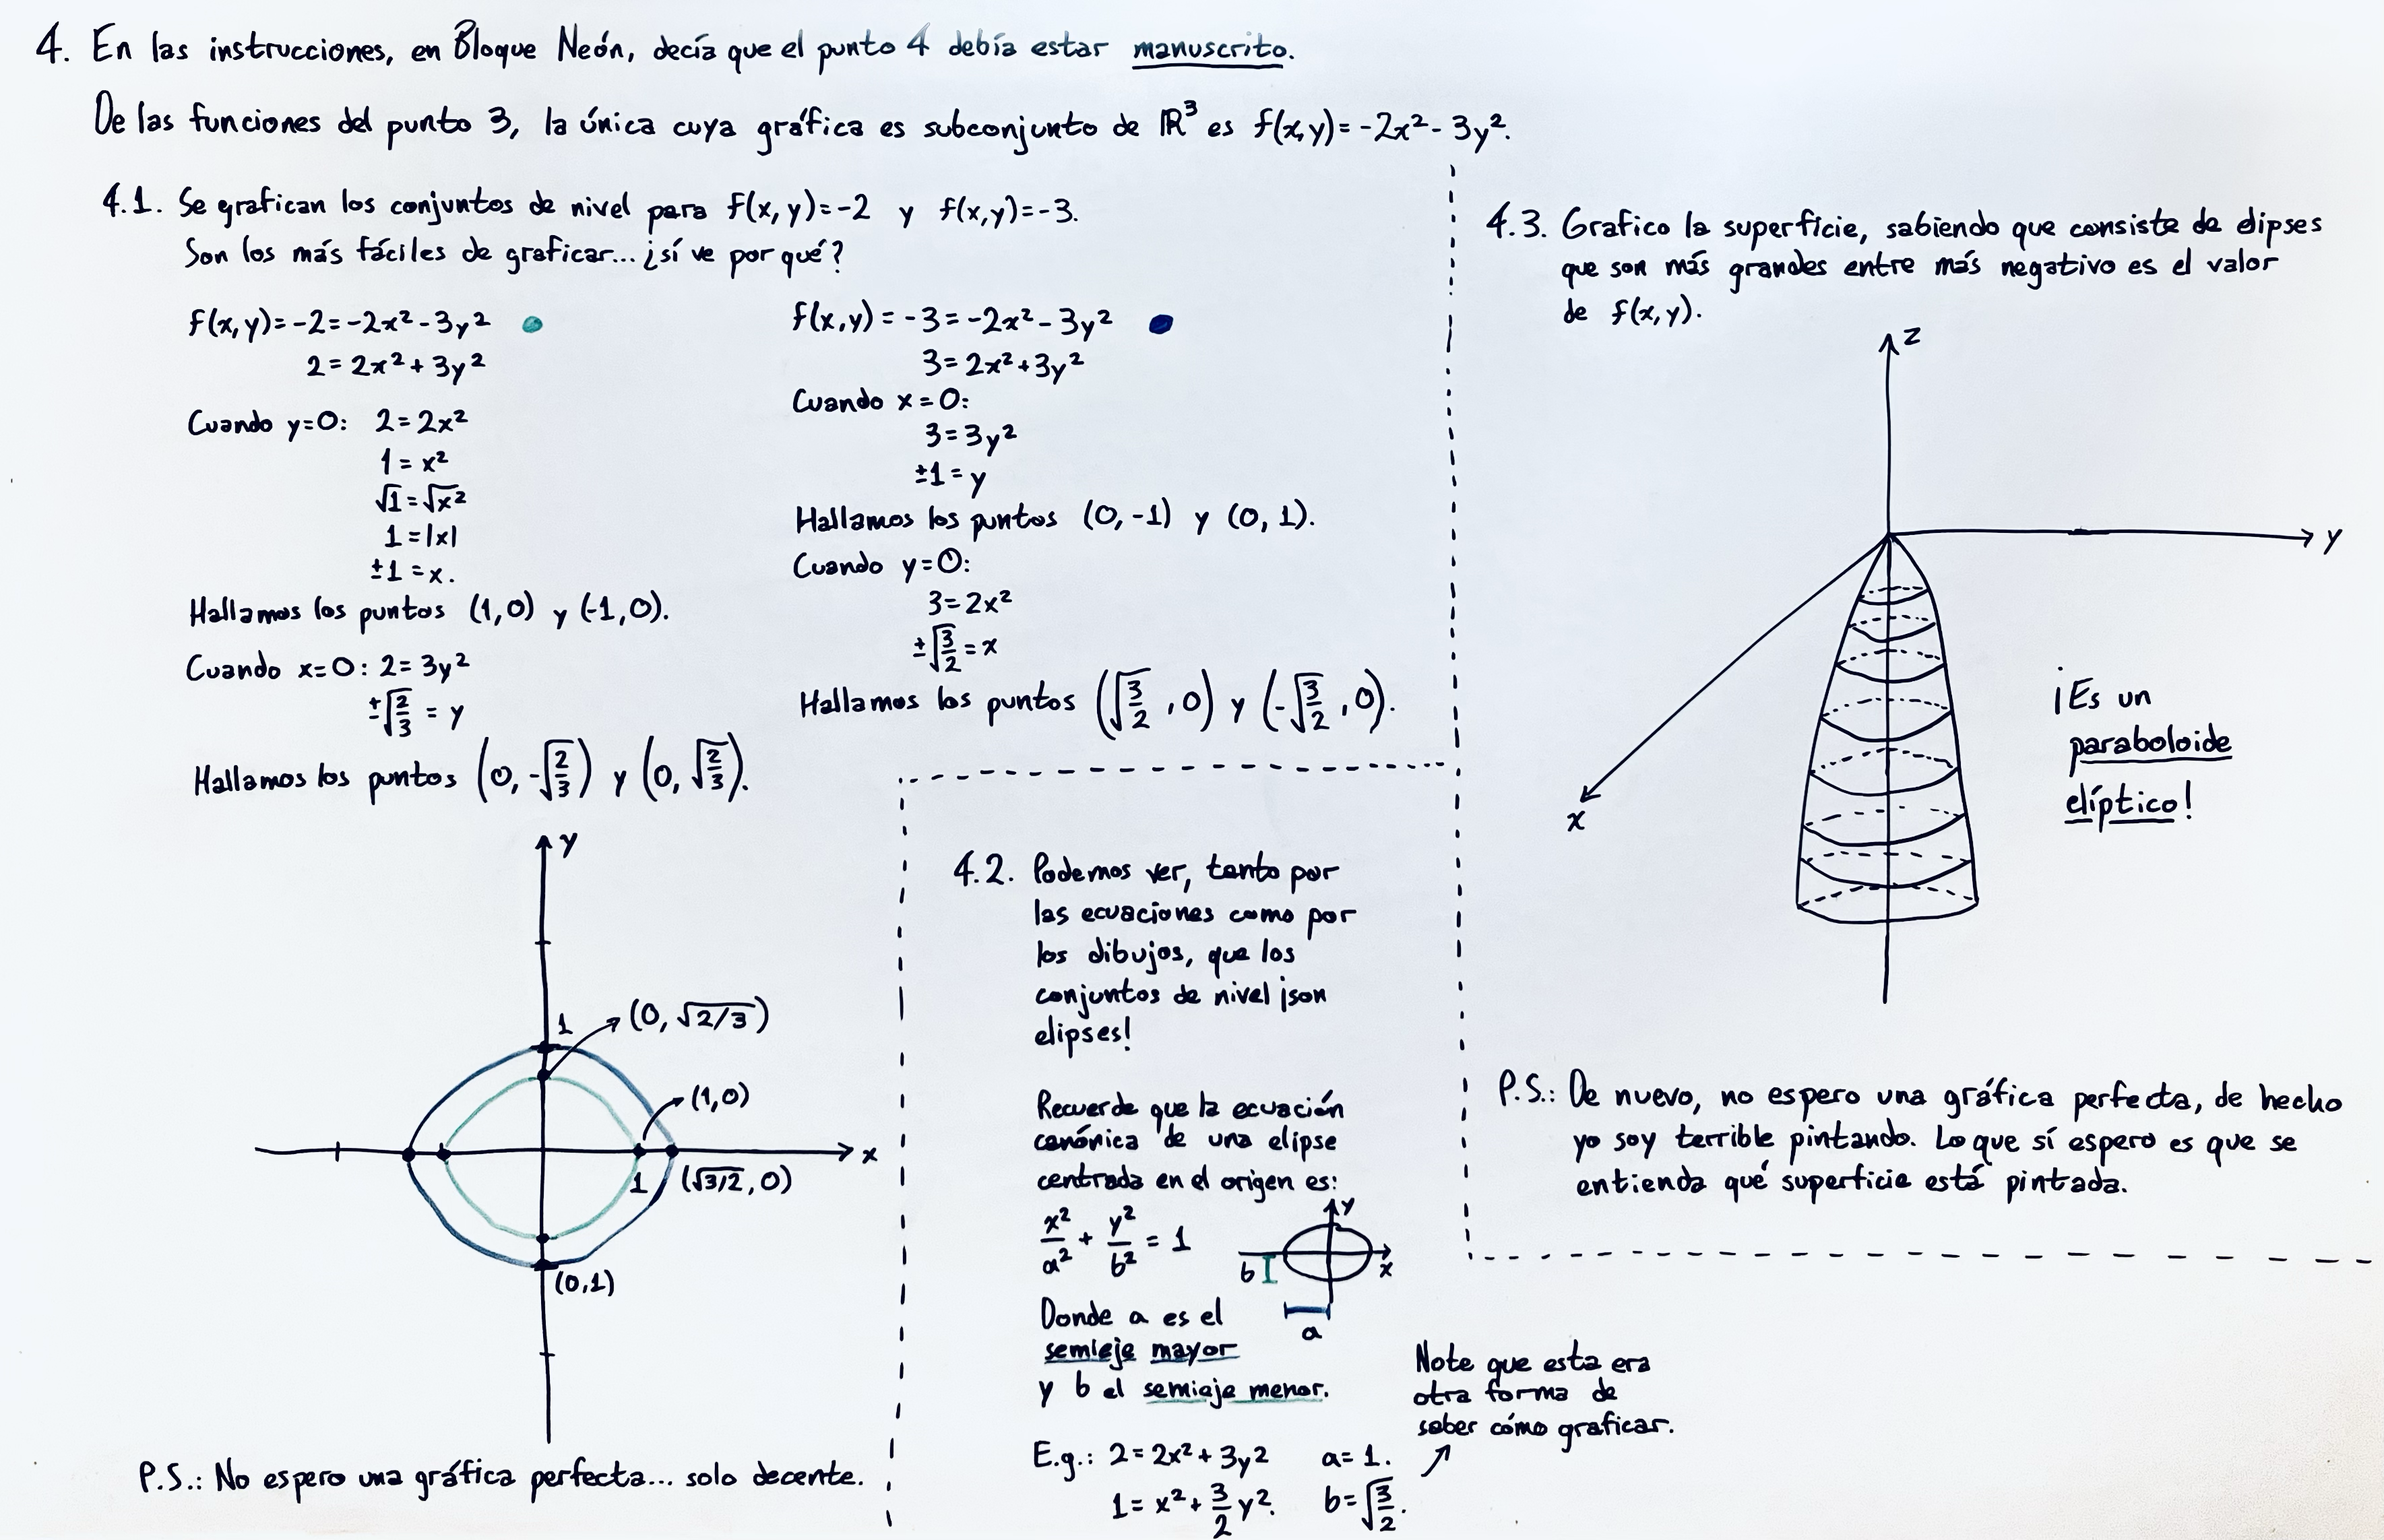
\includegraphics[width=1\textwidth]{punto4.png}

\end{problema}

% ---------------------------------------------------------------------------------------------------

\section{Límites}

\begin{problema}[Inexistencia de límites 1]

(\(0.\bar{3}\) puntos) Demuestre la existencia o inexistencia del siguiente límite.
     \[\displaystyle \lim_{(x, y) \to (1, 0)} \frac{(x-1)^2+2(x-1)y}{(x-1)y}.\]

\vspace{1em}
\tcblower
\textbf{Solución:}\\

Como dice en la guía para el cálculo de límites que se encuentra en Bloque Neón, algunas formas de abordar este problema (y el que le sigue) son evaluar el límite y realizar un cambio de variable usando coordenadas polares. Para este límite, tomar cualquiera de esos caminos resulta en una expresión que no proporciona información sobre el límite, es decir, no permite establecer si existe o no. Tras probar eso, la guía sugiere que una forma de demostrar la inexistencia del límite es acercándose al límite usando distintas direcciones. Se opta por ese procedimiento.\\

Primero, se simplifica el límite:
\begin{align*}
    \lim_{(x, y) \to (1, 0)} \frac{(x-1)^2+2(x-1)y}{(x-1)y} &= \lim_{(x, y) \to (1, 0)} \frac{(x-1)((x-1)+2y)}{(x-1)y}.
\end{align*}

Tras eso, se realiza el acercamiento al límite desde la dirección descrita por la función \(y = x+1\):
\begin{align*}
    \lim_{x \to 1} \frac{(x-1)((x-1)+2(x+1))}{(x-1)(x+1)} &= \lim_{x \to 1} \frac{(x-1)^2+2(x+1)(x-1)}{x^2+1} \\
    &= \lim_{x \to 1} \frac{(x-1)^2 + 2x^2 + 2}{x^2+1} \\
    & \stackrel{\text{H}}{=} \lim_{x \to 1} \frac{2(x-1) + 4x}{2x} \\
    &=  \frac{2(1-1) + 4(1)}{2(1)} \\
    &=  \frac{4}{2} \\
    &=  2.
\end{align*}


Se coloca una H encima del signo de igualdad para denotar el uso de la regla de L'Hôpital. \\

Similarmente, se realiza el acercamiento al límite desde otra dirección, esta vez la descrita por la función \(y = x-1\):
\begin{align*}
    \lim_{x \to 1} \frac{(x-1)((x-1)+2(x-1))}{(x-1)^2} &= \lim_{x \to 1} \frac{(x-1)^2(1+2)}{(x-1)^2} \\
    &= \lim_{x \to 1} \frac{3(x-1)^2}{(x-1)^2} \\
    & \stackrel{\text{H}}{=} \lim_{x \to 1} \frac{6(x-1)}{2(x-1)} \\
    & \stackrel{\text{H}}{=} \lim_{x \to 1} \frac{6}{2} \\
    & = 3.
\end{align*}

Se evidencia que al calcular los dos límites se obtienen resultados distintos. Por ende, como acercarse al límite original desde dos direcciones diferentes produce valores disímiles, se demuestra que \answ{el límite no existe}.
\qed

\end{problema}

\phantom{} % ---------------------------------------------------------------------------------------------------

\begin{problema}[Inexistencia de límites 2]

(\(0.\bar{3}\) puntos) Demuestre la existencia o inexistencia del siguiente límite.

     \[\displaystyle  \lim_{(x, y) \to (0, 0)} \frac{x^3+y^3}{xy}.\]

\vspace{1em}
\tcblower
\textbf{Solución:}\\

De forma similar al límite anterior, ni evaluar al límite ni realizar algún cambio de variable produce resultados dicientes. Por ende, se intenta un procedimiento análogo, acercándose al límite primero desde la dirección descrita por la función \(y = x\):
\begin{align*}
    \lim_{x \to 0} \frac{x^3+x^3}{xx} &=  \lim_{x \to 0} \frac{2x^3}{x^2} \\ 
    & \stackrel{\text{H}}{=} \lim_{x \to 0} \frac{6x}{2x} \\ 
    & \stackrel{\text{H}}{=} \lim_{x \to 0} \frac{6}{2} \\ 
    & = 3.
\end{align*}

Ahora, se toma la dirección descrita por la función \(y = x^2\). 
\begin{align*}
    \lim_{x \to 0} \frac{x^3+(x^2)^3}{x \, x^2} &=  \lim_{x \to 0} \frac{x^3(1+x^3)}{x^3} \\ 
    & = \lim_{x \to 0} 1+x^3\\
    & = 1.
\end{align*}
Puede parecer que las direcciones se seleccionan arbitrariamente, sin embargo, vale la pena elegir las direcciones pensando en qué tan laborioso resultará el reemplazo, sobretodo si la situación es apremiante (e.g., un examen). Por ejemplo, si para este límite se eligiese la dirección \(y = x+1\), el proceso resultaría más engorroso, pues sería necesario manipular el término \((x+1)^3\).\\

Al igual que en el ejercicio anterior, como acercarse al límite original desde dos direcciones diferentes produce valores disímiles, se demuestra que \answ{el límite no existe}.
\qed

\end{problema}

\section{Diferenciación}

\begin{problema}[Diferenciabilidad]
    (\(0.\bar{3}\) puntos) Demuestre o refute que \(f(x, y) = \cos(xy) +x\cos(y)\) es diferenciable para cualesquiera \(x, y \in \mathbb{R}\).

\vspace{1em}
\tcblower
\textbf{Solución:}\\

Se siguen prácticamente al pie de la letra los pasos del ejemplo resuelto de diferenciabilidad que se encuentra en Bloque Neón. \\

Se sabe de antemano que las funciones \(x\) y \(y\) son continuas, por lo cual su producto, \(xy\), es continuo también. Adicionalmente, se sabe que las funciones seno y coseno son continuas. Por ende, las composiciones \(\cos(xy)\) y \(\sin(xy)\) son continuas. Con eso en mente:\\

\begin{enumerate}
    \item Se demuestra primero que la función es continua en todo su dominio. \\ Se evidencia que \(f\) consiste de operaciones entre funciones continuas, por lo cual debe ser continua en todo su dominio.\\
    
    \item Se demuestra que \(\dparder[f(x, y)]\) es continua. \\\\ Se calcula la derivada parcial: \(\dparder[f(x, y)] = -y\sin(xy) + \cos(y)\). Similar a antes, se evidencia que  \(\dparder[f(x, y)]\) consiste de operaciones entre funciones continuas, por lo cual debe ser continua en todo su dominio.\\
    
    \item Se demuestra que \(\dparder[f(x, y)][y]\) es continua. \\\\  Igual que antes, se calcula la derivada parcial: \(\dparder[f(x, y)][y] =  -x\sin(xy) -x\sin(y) \). Nuevamente, se evidencia que la derivada parcial consiste de operaciones entre funciones continuas, por lo cual debe ser continua en todo su dominio.\\

    Habiendo mostrado que tanto la función como sus dos primeras derivadas parciales son continuas sobre todo \(\mathbb{R}^2\), se demuestra, por la condición suficiente para diferenciabilidad enunciada en el ejemplo resuelto de diferenciabilidad, que \(f(x, y) = \cos(xy) +x\cos(y)\) es diferenciable para cualesquiera \(x, y \in \mathbb{R}\). 
    \qed
\end{enumerate}

\end{problema}

\phantom{} % ---------------------------------------------------------------------------------------------------

\begin{problema}[Plano tangente]
    
    (\(0.\bar{3}\) puntos) Halle el plano que es tangente a la gráfica de \(g(x, y) = x^2+y^4+e^{xy}\) en el punto \((1, 0, 2)\). Elija y enuncie un punto \((x, y) \in \mathbb{R}^2\) en el que no haya un extremo de \(g\) y explique su elección.

\vspace{1em}
\tcblower
\textbf{Solución:}\\

Recuérdese que el gradiente de una función siempre es ortogonal a sus conjuntos de nivel. Por ende, una forma de determinar el plano tangente a una superficie en un punto, es tratar esa superficie como si fuese un conjunto de nivel de una función. Con eso, al hallar el gradiente de dicha función en el punto dado, se consigue un vector ortogonal a la superficie, que puede usarse como un vector normal del plano tangente. \\

Con eso en mente, primero se trata la superficie dada, \(g(x, y) = x^2+y^4+e^{xy}\), como un conjunto de nivel de la función \(f(x, y, z) = x^2+y^4+e^{xy}-z\). En este caso, es el conjunto de nivel que se obtiene cuando \(f(x, y, z) = 0\), pues
\begin{align*}
    0 &= x^2+y^4+e^{xy}-z \\
    z &= x^2+y^4+e^{xy} = g(x, y).
\end{align*}
    
Se busca entonces el gradiente de \(f\), que a continuación se calcula:
\begin{align*}
    \nabla f(\bvec{x}) &= \left( \dparder[f(\bvec{x})][x], \dparder[f(\bvec{x})][y], \dparder[f(\bvec{x})][z] \right) \\
    &= \left( 2x+y e^{xy}, 4y^3+x e^{xy}, -1 \right).
\end{align*}
Tras eso, se evalúa el gradiente en el punto al cual el plano que se busca debe ser tangente:
\begin{align*}
    \nabla f(1, 0, 2) &= \left( 2(1)+0 e^{(1)(0)} , 4(0)^3+1 e^{(1)(0)}, -1 \right).\\
    &= \left( 2, 1, -1 \right).
\end{align*}
Ese vector ejerce como un vector normal al plano que es tangente a la superficie de nivel \(g(x, y) = x^2+y^4+e^{xy}\) en el punto \((1, 0, 2)\). \\

Para obtener la ecuación del plano, recuérdese que el plano consta de todos los puntos que son perpendiculares al vector normal. Es decir, basta con una expresión que abarque todos los \((x, y, z)\) que sean ortogonales al vector normal, o lo que es lo mismo, que su producto punto con el vector normal sea igual a \(0\):
\begin{gather*}
    (2, 1, -1) \cdot (x, y, z) = 0 \\
    2x + y - z = 0 \\
    z = 2x + y.
\end{gather*}
Así pues, el plano que es tangente a la gráfica de \(g(x, y) = x^2+y^4+e^{xy}\) en el punto \((1, 0, 2)\) es
\begin{gbox}
    \[z = 2x + y.\]
\end{gbox}

Para finalizar, se pide elegir y enunciar un punto \((x, y) \in \mathbb{R}^2\) en el cual no haya un extremo de \(g\). Si se entienden con claridad los conceptos del curso, tras determinar el plano tangente, debió ser inmediatamente claro que un punto que satisface esa condición es el dado por el enunciado, \((1, 0)\). \\

Eso se debe a que para que un punto \((x, y, z)\) sea extremo de una función \(h\colon \mathbb{R}^2 \to \mathbb{R}\), el plano tangente a la función en ese punto debe ser paralelo al plano \(xy\). Es decir, la ecuación del plano tangente debe ser de la forma \(z = c\), con \(c \in \mathbb{R}\). Esto es análogo a lo que se estudia en clase de Cálculo Diferencial: en ese curso, para que un punto sea extremo de una función, la recta tangente a la función en ese punto debe ser horizontal, paralela al eje \(x\). \\

Dicho eso,
\begin{gbox}
    Un punto en el que no hay un extremo de \(g\) es \((1, 0)\), debido a que el plano que es tangente a \(g\) en \((1, 0, 2)\) no es paralelo al plano \(xy\).
\end{gbox}
 
\end{problema}

\phantom{} % ---------------------------------------------------------------------------------------------------

\begin{problema}[Pedro]
    (\(0.\bar{3}\) puntos) Pedro es un extraterrestre de uno de los satélites de Saturno, Titán. Pedro precisa de altas concentraciones de nitrógeno para su supervivencia. La concentración percibida de nitrógeno con respecto a la ubicación en Titán está modelada por la función \(N(x, y, z) = x^2+y^4+2z^2\), donde \(x\), \(y\) y \(z\) están medidas en decámetros y \(N(x, y, z)\) está medida en \(\mathrm{mg} \, \mathrm{L}^{-1}\). \\
    
    Pedro se está empezando a sentir sofocado por carencia de nitrógeno. Decide desplazarse en línea recta en la dirección en la que la concentración de nitrógeno incrementa más rápidamente. Si él sabe que está ubicado en el punto \((1, 1, 1)\), ¿en qué dirección debe avanzar en aras de convalecerse? Al desplazarse en esa dirección, ¿cuál es la tasa de cambio de la concentración de nitrógeno?
    \begin{figure}[H]
        \centering
        \includegraphics[width=0.3\textwidth]{marciano.png}
        \caption{Pedro.}
    \end{figure}

\vspace{1em}
\tcblower
\textbf{Solución:}\\


Para ayudar a Pedro a convalecerse, se busca determinar la dirección en la que la concentración de nitrógeno incrementa más rápidamente. Como la concentración de nitrógeno con respecto a la ubicación en Titán está modelada por la función \(N(x, y, z) = x^2+y^4+2z^2\), y recordando que el gradiente de una función apunta en la dirección a lo largo de la cual la función crece más rápidamente, para hallar la dirección buscada basta con calcular el gradiente de \(N\), evaluarlo en el punto en el que se encuentra Pedro y obtener su vector unitario, que es la dirección como tal. \\

Se calcula el gradiente:
\begin{align*}
    \nabla N(\bvec{x}) &= \left( \dparder[N(\bvec{x})][x], \dparder[N(\bvec{x})][y], \dparder[N(\bvec{x})][z] \right) \\
    &= \left( 2x, 4y^3, 4z\right).
\end{align*}
Se evalúa el gradiente en la ubicación de Pedro, que es \((1, 1, 1)\):
\begin{align*}
    \nabla N((1, 1, 1)) &= \left( 2(1), 4(1)^3, 4(1)\right) \\
    &= \left( 2, 4, 4\right).
\end{align*}
Por último, se computa el vector unitario, dividiendo el vector por su norma:
\begin{align*}
    &= \frac{( 2, 4, 4)}{\norm{(2, 4, 4)}} \\
    &= \frac{( 2, 4, 4)}{\sqrt{2^2 + 4^2 + 4^2}} \\
    &= \frac{( 2, 4, 4)}{\sqrt{4 + 16 + 16}} \\
    &= \frac{( 2, 4, 4)}{\sqrt{36}}\\
    &= \frac{( 2, 4, 4)}{6}\\
    &= \left( \frac{1}{3}, \frac{2}{3}, \frac{2}{3}\right).
\end{align*}
Esa es la dirección que debe seguir Pedro. Para ser más puntuales, 
\begin{gbox}
    Pedro debe desplazarse siguiendo la semirecta \[\begin{pmatrix}
        1 \\ 1 \\ 1
    \end{pmatrix} + t\begin{pmatrix}
        1/3 \\ 2/3 \\ 2/3
        \end{pmatrix}, \quad t\in \mathbb{R}_{>0}. \]
    donde \(t\) está medida en decámetros.
\end{gbox}

La tasa de cambio de la concentración de nitrógeno está dada por la magnitud del gradiente en el punto \((1, 1, 1)\), que es la norma calculada recién, \(\norm{(2, 4, 4)}\), y es igual a 6.
\begin{gbox}
    La tasa de cambio de la concentración de nitrógeno es \[6 \ \text{mg} \, \text{L}^{-1} \, \text{dam}^{-1}. \]
\end{gbox}
La unidades representan que por cada decámetro recorrido, la concentración de nitrógeno incrementa en \(6 \ \text{mg} \, \text{L}^{-1}\). Se puede pensar en esta unidad de forma análoga a como se piensa en la unidad cotidiana de velocidad, los kilómetros por hora, \( \text{km} / \text{h} = \text{km} \, \text{h}^{-1}\). La expresión \( 1 \, \text{km} \, \text{h}^{-1}\) representa que por cada hora de trayecto, la distancia recorrida incrementa en \( 1 \, \text{km} \).

\end{problema}

% ---------------------------------------------------------------------------------------------------

\section{Optimización}

\begin{problema}[]
    (\(0.\bar{3}\) puntos)  Enuncie dos métodos distintos para hallar los extremos locales de una función restringida a un compacto. ¿Existen circunstancias bajo las cuáles un método es preferible al otro? Si sí, provea un ejemplo; de lo contrario, explique su raciocinio.


\vspace{1em}
\tcblower
\textbf{Solución:}\\

    Hay una infinidad de respuestas correctas para esta pregunta, que incluso podría considerarse una pregunta de opinión. Su propósito era hacerlos reflexionar sobre cómo se puede abordar un problema de diferentes maneras, algo que es muy común en matemáticas. Marcaré como correcta cualquier respuesta con una explicación coherente. \\

    El único comentario que quiero hacer frente a esta pregunta es que catalogar un método matemático como \textit{preferible} en comparación con otro suscita inmediatamente interrogantes como ¿preferible para qué? o ¿preferible para quién? Podría argüirse que, para un individuo arbitrario, el mejor método matemático es aquel que mejor entiende, basado en su conocimiento previo y sus habilidades.
\end{problema}

\phantom{} % ---------------------------------------------------------------------------------------------------

\begin{problema}[optimización]

    (\(0.\bar{3}\) puntos)  Dada la función \(f(x,y)=x^2+y^2-2y\) definida en el disco \(x^2+y^2\leq 4\), indique cuáles son los extremos de la función en ese disco. 

\vspace{1em}
\tcblower
\textbf{Solución:}\\

    En este problema resulta evidente que la función objetivo es \(f(x,y)=x^2+y^2-2y\) y que la restricción es \(g(x, y) = x^2+y^2 \leq 4\). Primeramente, para determinar los puntos críticos de \(f\), se calcula su gradiente:
    \begin{align*}
        \nabla f(x,y) &= \left( \dparder[f(x,y)][x], \dparder[f(x,y)][y] \right) \\
    &= \left( 2x, 2y-2\right)
    \end{align*}
    Tras eso, se iguala el gradiente al vector cero, análogamente a como se hace en el ejercicio de repaso de Cálculo Diferencial:
    \begin{gather*}
        \left( 2x, 2y+2\right) = (0, 0) \\
        \begin{cases}
            2x = 0 \\
            2y-2 = 0
        \end{cases} \\
        \begin{cases}
            x = 0 \\
            y = 1.
        \end{cases}
    \end{gather*}


    El único punto crítico es \((0, 1)\). Antes de determinar si es un máximo o un mínimo, se verifica que se encuentre dentro del disco, pues de lo contrario es irrelevante para el problema.
    \begin{align*}
        x^2+y^2 &\leq 4 \\
        0^2+1^2 &\leq 4 \\
        1 &\leq 4.
    \end{align*}

    Tras confirmar que el punto crítico es relevante, para determinar si el punto crítico es un extremo, debe recordarse el criterio del determinante de la matriz hessiana. Recuérdese que dicho determinante está dado por
    \begin{equation*}
        \begin{vmatrix}
            \dnparder{2}[f][x] & \dfrac{\partial^2 f}{\partial x \partial y} \\[2ex]
            \dfrac{\partial^2 f}{\partial y \partial x} & \dnparder{2}[f][y]
        \end{vmatrix} = \left(\nparder{2}[f][x]\right)\left(\nparder{2}[f][y]\right) - \left(\frac{\partial^2 f}{\partial x \partial y}\right)^2.
    \end{equation*}
    Y el criterio asociado a él es el siguiente:
    \begin{itemize}
        \item Si \(\displaystyle \left(\nparder{2}[f(\bvec{v})][x]\right)\left(\nparder{2}[f(\bvec{v})][y]\right) - \left(\frac{\partial^2 f(\bvec{v})}{\partial x \partial y}\right)^2 >0 \), existe un extremo en \(f(\bvec{v})\).
        \begin{itemize}
        \item Si \(\displaystyle \nparder{2}[f(\bvec{v})][x] > 0 \), entonces \(f(\bvec{v})\) es un mínimo.
        \item Si \(\displaystyle \nparder{2}[f(\bvec{v})][x] < 0 \), entonces \(f(\bvec{v})\) es un máximo. 
        \end{itemize}
        \item  Si \(\displaystyle \left(\nparder{2}[f(\bvec{v})][x]\right)\left(\nparder{2}[f(\bvec{v})][y]\right) - \left(\frac{\partial^2 f(\bvec{v})}{\partial x \partial y}\right)^2 <0 \), hay un punto de silla \(f(\bvec{v})\).
        \item  Si \(\displaystyle \left(\nparder{2}[f(\bvec{v})][x]\right)\left(\nparder{2}[f(\bvec{v})][y]\right) - \left(\frac{\partial^2 f(\bvec{v})}{\partial x \partial y}\right)^2 = 0 \), es un punto crítico degenerado, por lo que no se puede afirmar nada sobre el comportamiento de la función en ese punto.\\
    \end{itemize}
    
    En este caso, el cálculo del determinante es
    \begin{align*}
        \left(\nparder{2}[f][x]\right)\left(\nparder{2}[f][y]\right) - \left(\frac{\partial^2 f}{\partial x \partial y}\right)^2 = (2)(2) - 0 = 4 > 0.
    \end{align*}
    Por lo cual existe un extremo en \((0, 1)\). Sumado a eso, 
    \begin{align*}
        \left(\nparder{2}[f][x]\right) = 2 > 0,
    \end{align*}
    por lo cual en \((0, 1)\) hay un mínimo. El valor de dicho mínimo es
    \begin{align*}
        f(0, 1) = -1.
    \end{align*}
    Se concluye entonces que
    \begin{gbox}
        La función \(f\) restringida al disco \(x^2+y^2\leq 4\) tiene un mínimo en el punto \((0, 1)\) cuyo valor es \(-1\).
    \end{gbox}

    Ahora, se evalúan los puntos críticos en el borde del disco. Para ello, se utiliza el método de multiplicadores de Lagrange, que permite plantear la siguiente expresión:
    \begin{align*}
        &\begin{cases}
            \nabla f(\bvec{x}) = \lambda \nabla g(\bvec{x}) \\
            x^2 + y^2 = 4
        \end{cases} \\
        &\begin{cases}
            (2x, 2y-2) = \lambda (2x, 2y) \\
            x^2 + y^2 = 4
        \end{cases} \\
        &\begin{cases}
            2x = \lambda 2x \\
            2y-2 = \lambda 2y \\
            x^2 + y^2 = 4
        \end{cases}
    \end{align*}
    Para solucionar ese sistema de ecuaciones, supóngase primero que \(x \neq 0\). En ese caso, se puede despejar \(\lambda\) de la primera ecuación como \(\lambda = \frac{2x}{2x} = 1\). Eso se puede reemplazar en la segunda ecuación:
    \begin{align*}
        2y-2 &= \lambda 2y \\
        2y-2 &= 2y \\
        2y-2y &= 2 \\
        0 &= 2,
    \end{align*}
    Como eso es una inconsistencia, se sabe entonces que la suposición realizada es falsa y necesariamente \(x = 0\). Con eso, se puede resolver inmediatamente la tercera ecuación del sistema,
    \begin{align*}
        x^2 + y^2 &= 4 \\
        y^2 &= 4 \\
        \sqrt{y^2} &= \sqrt{4} \\
        |y| &= 2 \\
        y &= \pm 2.
    \end{align*}
    Se tienen entonces otros dos puntos en los que existen extremos cuando la función se restringe exclusivamente al borde del compacto. Se evalúan estos puntos en la función para compararlos con el punto crítico que ya se conoce,
    \begin{align*}
        f(0, -2) = 0+4-2(-2) = 8 \\
        f(0, 2) = 0+4-2(2) = 0.
    \end{align*}
    Con eso en mente, se puede concluir lo siguiente:
    \begin{gbox}
        La función \(f(x,y)=x^2+y^2-2y\) restringida al disco \(x^2+y^2\leq 4\) tiene un \answ{mínimo} en \((0, 1)\) cuyo valor es \(-1\) y un \answ{máximo} en \((0, -2)\) cuyo valor es \(8\).
    \end{gbox}
    
\end{problema}

\phantom{} % ---------------------------------------------------------------------------------------------------

\begin{problema}[Optimización identificando la función a optimizar]
    
    (\(0.\bar{3}\) puntos)  De todos los puntos contenidos en \(y\sqrt{x} = \sqrt{2}\) indique cuál es el más cercano al origen.

\vspace{1em}
\tcblower
\textbf{Solución:}\\

El primer paso para resolver este problema es identificar que es un problema de optimización. Una forma de identificar eso es percatarse de que el problema está ubicado en la sección de Optimización del enunciado. Otra forma, más general, es notar que el punto de la superficie \(y\sqrt{x} = \sqrt{2}\) que es más cercano al origen se puede interpretar como el punto mínimo de la función que mide la distancia entre el origen y la función \(y\sqrt{x} = \sqrt{2}\).\\

La fórmula que mide la distancia en \(\mathbb{R}^2\) entre dos puntos \((x,y)\) y \((\hat{x},\hat{y})\) es \(\sqrt{(x-\hat{x})^2+(y-\hat{y})^2}\). Si uno de esos puntos es el origen, la fórmula se reduce a \(\sqrt{x^2+y^2}\). Optimizar esa función es equivalente a optimizar la función \(f(x, y) = x^2+y^2\), por lo cual se toma esa como la función objetivo para este problema. Para la optimización, se debe tener en cuenta que se busca un punto en la función \(g(x, y) = y\sqrt{x} = \sqrt{2}\), por lo que la optimización debe estar restringida a ella. \\

Se utiliza el método de multiplicadores de Lagrange. Se tiene:
\begin{align*}
    &\begin{cases}
        \nabla f(\bvec{x}) = \lambda \nabla g(\bvec{x}) \\
        y\sqrt{x} = \sqrt{2}.
    \end{cases} \\
    &\begin{cases}
        (2x, 2y) = \lambda (\frac{1}{2}y \, x^{-\frac{1}{2}}, \sqrt{x}) \\
        y\sqrt{x} = \sqrt{2}.
    \end{cases} \\
    &\begin{cases}
        2x = \lambda \frac{y}{2\sqrt{x}} \\
        2y = \lambda \sqrt{x} \\
        y\sqrt{x} = \sqrt{2}.
    \end{cases}
\end{align*}

Nótese del sistema de ecuaciones anterior que \(x > 0\), pues de lo contrario es imposible satisfacer \(y\sqrt{x} = \sqrt{2}\). Por la misma razón se sabe también que \(y \neq 0\). Con eso en mente, que es indispensable para poder dividir por cualquiera de las variables, se despeja \(\lambda\) de la segunda ecuación del sistema:
\begin{align*}
    2y &= \lambda \sqrt{x} \\
     \lambda &= \frac{2y}{\sqrt{x}},
\end{align*}
y se despeja \(y\) de la tercera ecuación del sistema:
\begin{align*}
    y\sqrt{x} &= \sqrt{2} \\
    y &= \sqrt{\frac{2}{x}}.
\end{align*}
Con eso, se reemplazan ambos valores en la primera ecuación del sistema. Primero,  \(\lambda\):
\begin{align*}
    2x &= \frac{2y}{\sqrt{x}} \cdot \frac{y}{2\sqrt{x}} \\
    2x &= \frac{2y^2}{2x} \\
    4x^2 &= 2y^2 \\
    2x^2 &= y^2,
\end{align*}
y luego, \(y\):
\begin{align*}
    2x^2 &= \sqrt{\frac{2}{x}}^2 \\
    2x^2 &= \frac{2}{x}\\
    2x^3 &= 2 \\
    x^3 &= 1 \\
    x &= 1.
\end{align*}
Para finalizar, se reemplaza \(x\) en la expresión que ya se conoce para \(y\):
\begin{align*}
    y &= \sqrt{\frac{2}{x}} \\
    y &= \sqrt{\frac{2}{1}} \\
    y &= \sqrt{2}.
\end{align*}

Con ese procedimiento, se determina que:
\begin{gbox}
    El punto en \(y\sqrt{x} = \sqrt{2}\) más cercano al origen es \((1, \sqrt{2})\).
\end{gbox}

\end{problema}

\phantom{} % ---------------------------------------------------------------------------------------------------

\begin{problema}[Optimización de volumen]
    
    (\(0.\bar{3}\) puntos) Suponga que cuenta con \(12 \, \mathrm{cm}^2 \) de cartón que usará como material para las paredes y el piso de una caja rectangular sin tapa. Desprecie la forma en la que unirá las paredes entre sí y no contemple tampoco el grosor del cartón.
    \begin{itemize}
        \item Dibuje una caja que podría armar con ese material sin desperdiciar material. Indique las dimensiones de la caja en el dibujo.
        \item Dibuje la caja que se puede armar con ese material que maximice el volumen de líquido que puede contener. Indique las dimensiones de esta caja en el dibujo. Explique por qué está seguro de que, bajo las mismas condiciones, no se puede construir otra caja de mayor volumen.
    \end{itemize}
    \begin{figure}[H]
        \centering
        \includegraphics[width=0.5\textwidth]{caja.png}
        \caption{Dibujo de una caja rectangular sin tapa con sus dimensiones indicadas, construida con \(41 \, \mathrm{cm}^2 \) de cartón. Note que el dibujo no está a escala; el suyo tampoco debe estarlo.}
    \end{figure}
        

\vspace{1em}
\tcblower
\textbf{Solución:}\\

Para el primer inciso de este problema, se pide una caja sin tapa que sea posible armar con \(12 \, \mathrm{cm}^2 \) de cartón, sin desperdiciar material. Es decir, se busca cualquier prisma rectangular incompleto, de cinco caras, cuya área superficial sean \(12 \, \mathrm{cm}^2 \). Una forma fácil de obtener dimensiones que satisfagan esa condición es que todas las dimensiones del prisma sean iguales, denotadas por \(x\). En ese caso, basta con resolver la ecuación
\begin{align*}
    5x^2 &= 12 \\
    x^2 &= \frac{12}{5} \\
    \sqrt{x^2} &= \sqrt{\frac{12}{5}} \\
    |x| &= \sqrt{\frac{12}{5}}.
\end{align*}
Esa ecuación indica que \(\sqrt{\frac{12}{5}} \, \mathrm{cm}\) es una medida apropiada para cada lado. Un dibujo de una caja en la que todas las dimensiones son \(\sqrt{\frac{12}{5}} \, \mathrm{cm}\) es el siguiente:

\begin{gbox}
    \begin{figure}[H]
        \centering
        \includegraphics[width=0.3\textwidth]{caja12.png}
        \caption{Caja sin techo en la que todas las dimensiones son \(\sqrt{\frac{12}{5}} \, \mathrm{cm}\), construida con \(12 \, \mathrm{cm}^2 \) de material.}
    \end{figure}
\end{gbox}

Para el segundo inciso de este problema sí es necesario emplear herramientas del cálculo. Se busca maximizar el volumen de la caja, que está dado por la función \(f(x, y, z)=xyz\). Además de eso, se necesita que el área superficial sea exactamente \(12 \, \mathrm{cm}^2 \), para lo cual se puede establecer que \(g(x, y, z)=xy + 2yz + 2xz = 12\). Con eso, se puede utilizar el método de multiplicadores de Lagrange para hallar los extremos de \(f\) restringida a \(g(x, y) = 12\):
\begin{align*}
    &\begin{cases}
        \nabla f(\bvec{x}) = \lambda \nabla g(\bvec{x}) \\
        xy + 2yz + 2xz = 12.
    \end{cases} \\
    &\begin{cases}
        (yz, xz, xy) = \lambda (y + 2z, x + 2z, 2y + 2x) \\
        xy + 2yz + 2xz = 12.
    \end{cases} \\
    &\begin{cases}
        yz = \lambda(y + 2z) \\
        xz = \lambda(x + 2z) \\
        xy = \lambda(2y + 2x) \\
        xy + 2yz + 2xz = 12.
    \end{cases}
\end{align*}

Para resolver este sistema de ecuaciones, se puede sacar provecho de que se sabe que \(x\), \(y\) y \(z\) son las dimensiones de una caja, y por ende \(x > 0\), \(y > 0\) y \(z > 0\). Eso permite dividir por cualquiera de las variables y descartar las soluciones negativas. Con eso en mente, se despeja \(\lambda\) de las primeras dos ecuaciones del sistema y se igualan entre sí:
\begin{align*}
    yz = \lambda(y + 2z) \quad & \quad  xz = \lambda(x + 2z)\\
    \lambda = \frac{yz}{y + 2z} \quad & \quad  \lambda = \frac{xz}{x + 2z}\\
    \frac{yz}{y + 2z} &= \frac{xz}{x + 2z}\\
    (yz)(x + 2z) &= (xz)(y + 2z) \\
    xyz + 2yz^2 &= xyz + 2xz^2 \\
    xy + 2yz &= xy + 2xz \\
    yz &=  xz \\
    y &=  x.
\end{align*}
Luego, se realiza un proceso similar con las ecuaciones primera y tercera del sistema, pero sacando provecho de que \(x=y\) para reemplazar \(y\) por \(x\)
\begin{align*}
    yz = \lambda(y + 2z) \quad & \quad  xy = \lambda(2y + 2x)\\
    \lambda = \frac{yz}{y + 2z} \quad & \quad  \lambda = \frac{xy}{2y + 2x}\\
    \frac{yz}{y + 2z} &= \frac{xy}{2y + 2x}\\
    \frac{xz}{x + 2z} &= \frac{x^2}{2x + 2x}\\
    (xz)(2x + 2x) &= (x^2)(x + 2z)\\
    2x^2z + 2x^2z &= x^3 + 2x^2z\\
    2x^2z &= x^3 \\
    2z &= x \\
    z &= \frac{x}{2}.
\end{align*}
En este punto, se conocen expresiones para todas las dimensiones en términos de \(x\). Se reemplazan en la expresión del área superficial para determinar el valor de \(x\) y con eso a su vez el valor de las dimensiones:
\begin{align*}
    xy + 2yz + 2xz &= 12 \\
    xx + 2x\frac{x}{2} + 2x\frac{x}{2} &= 12 \\
    3x^2 &= 12 \\
    x^2 &= 4 \\
    \sqrt{x^2} &= \sqrt{4} \\
    |x| &= 2 \\
    x &= 2.
\end{align*}
Se remueve el valor absoluto sin contemplaciones puesto que se sabe de antemano que \(x > 0\). Sabiendo que \(x = 2\), se sabe también que \(y = 2\) y que \(z = \frac{2}{2} = 1\). Esos valores representan las dimensiones de la caja, medidos en centímetros. Ergo:
\begin{gbox}
    Las dimensiones óptimas son \(2 \, \text{cm} \times 2 \, \text{cm} \times 1 \, \text{cm} \).
\end{gbox}
Eso produce el siguiente dibujo:

\begin{gbox}
    \begin{figure}[H]
        \centering
        \includegraphics[width=0.3\textwidth]{caja-optima.png}
        \caption{Caja sin techo de volumen máximo, de todas las que pueden ser construidas con \(12 \, \mathrm{cm}^2 \) de material.}
    \end{figure}
\end{gbox}

Respecto al último inciso de esta pregunta, sobre por qué estamos seguros de que la caja pintada recién efectivamente representa la de mayor volumen y no existe alguna otra que la desbanque como la óptima, es una pregunta con un componente epistemológico. ¿Cómo sabemos que la matemática, en general, como disciplina, es correcta? Al igual que en el punto 10, marcaré como correcta cualquier respuesta que ofrezca una explicación coherente al respecto.

\end{problema}

% ---------------------------------------------------------------------------------------------------

\section{Funciones con valores vectoriales}

\begin{problema}[Cinemática]

    Sea \(\sigma\colon [0,2] \to \mathbb{R}^{3}\) la trayectoria dada por \(\sigma (t) = \left(1,t,\frac{t^3}{3}\right)\) donde las unidades de distancia son los metros y \(t\) está medida en segundos.
    \begin{enumerate}[label=14.\arabic*]
        \itemp[\(0.\bar{1}\)] Indique la velocidad.
        \itemp[\(0.\bar{1}\)] Indique la rapidez.
         \itemp[\(0.\bar{1}\)] Indique la longitud de la trayectoria.
    \end{enumerate}

    
\vspace{1em}
\tcblower
\textbf{Solución:}\\

    Teniendo en cuenta que la función representa una trayectoria, la velocidad está dada por la primera derivada de la función con respecto al tiempo:
    \begin{gbox}
        \begin{equation*}
            \sigma' (t) = (0,1,t^2) \, \text{m} \, \text{s}^{-1}.
        \end{equation*}
    \end{gbox}
    

    La rapidez es la magnitud de la velocidad, es decir: 
    \begin{gbox}
        \begin{equation*}
            \norm{\sigma' (t)} = \sqrt{1+t^4} \, \text{m} \, \text{s}^{-1}.
        \end{equation*}
    \end{gbox}
    
   Por último, la longitud de la trayectoria equivale a la longitud de arco de la trayectoria:	
    \begin{gbox}
        \begin{equation*}
            L (\sigma) = \defint{\sqrt{1+t^4}}[t]{0}{2} \, \text{m}.
        \end{equation*}
    \end{gbox}
    P.S.: Como varios notaron, hallar un valor numérico para esta integral no es nada fácil. Como les dije a todos los que preguntaron, es suficiente con que la integral esté expresada.
\end{problema}

% ---------------------------------------------------------------------------------------------------

\section{Funciones con valores vectoriales}

\begin{problema}[Propiedad de Campos vectoriales]
    (\(0.\bar{3}\) puntos) Sea \(U \subseteq \mathbb{R}^{m}\) un conjunto abierto y sean \(\bvec{F},\bvec{G}\colon U\to \mathbb{R}^{n}\) campos vectoriales. Demuestre o refute la siguiente propiedad:
\[\div (\bvec{F} \times \bvec{G}) = \nabla \cdot (\bvec{F} \times \bvec{G}) = \bvec{G}\cdot \rot\bvec{F} - \bvec{F}\cdot \rot \bvec{G}.\]
\tcblower
\textbf{Solución:}\\

Primeramente, nótese que para que el producto cruz esté bien definido, es necesario que \(n = m = 3\). \\

Con eso en mente, se definen los campos vectoriales como
\begin{gather*}
    \bvec{F} = (\bvec{F}_1, \bvec{F}_2, \bvec{F}_3) \\
    \bvec{G} = (\bvec{G}_1, \bvec{G}_2, \bvec{G}_3).
\end{gather*}

Como primera etapa de la prueba, se calcula la divergencia:
\begin{align*}
    \div (\bvec{F} \times \bvec{G}) &= \nabla \cdot (\bvec{F} \times \bvec{G}) \\
    &= \nabla \cdot \begin{vmatrix}
        \uvec{i} & \uvec{j} & \uvec{k} \\
        \bvec{F}_1 & \bvec{F}_2 & \bvec{F}_3 \\
        \bvec{G}_1 & \bvec{G}_2 & \bvec{G}_3
    \end{vmatrix} \\
    &= \nabla \cdot (\bvec{F}_2 \bvec{G}_3 - \bvec{F}_3 \bvec{G}_2, \bvec{F}_3 \bvec{G}_1 - \bvec{F}_1 \bvec{G}_3, \bvec{F}_1 \bvec{G}_2 - \bvec{F}_2 \bvec{G}_1) \\
    &= \left(\frac{\partial}{\partial x},\frac{\partial}{\partial y},\frac{\partial}{\partial z}\right) \cdot (\bvec{F}_2 \bvec{G}_3 - \bvec{F}_3 \bvec{G}_2, \bvec{F}_3 \bvec{G}_1 - \bvec{F}_1 \bvec{G}_3, \bvec{F}_1 \bvec{G}_2 - \bvec{F}_2 \bvec{G}_1) \\
    &= \frac{\partial}{\partial x}(\bvec{F}_2 \bvec{G}_3 - \bvec{F}_3 \bvec{G}_2) + \frac{\partial}{\partial y}(\bvec{F}_3 \bvec{G}_1 - \bvec{F}_1 \bvec{G}_3) + \frac{\partial}{\partial z}(\bvec{F}_1 \bvec{G}_2 - \bvec{F}_2 \bvec{G}_1) \\
    &= \frac{\partial \bvec{F}_2 \bvec{G}_3}{\partial x} - \frac{\partial \bvec{F}_3 \bvec{G}_2}{\partial x} + \frac{\partial \bvec{F}_3 \bvec{G}_1}{\partial y} - \frac{\partial \bvec{F}_1 \bvec{G}_3}{\partial y} + \frac{\partial \bvec{F}_1 \bvec{G}_2}{\partial z} - \frac{\partial \bvec{F}_2 \bvec{G}_1}{\partial z}
\end{align*}
Esa expresión se puede extender haciendo uso de la regla del producto de la derivación, \((fg)' = f'g + fg'\). Con eso, se tiene:
\begin{align*}
    \div (\bvec{F} \times \bvec{G}) = \ & \bvec{G}_3\frac{\partial \bvec{F}_2}{\partial x} + \bvec{F}_2\frac{\partial  \bvec{G}_3}{\partial x} - \bvec{G}_2\frac{\partial \bvec{F}_3 }{\partial x} - \bvec{F}_3\frac{\partial \bvec{G}_2}{\partial x} + \bvec{G}_1\frac{\partial \bvec{F}_3}{\partial y} + \bvec{F}_3\frac{\partial \bvec{G}_1}{\partial y} \\ & - \bvec{F}_1\frac{\partial \bvec{G}_3}{\partial y} - \bvec{G}_3\frac{\partial \bvec{F}_1}{\partial y} + \bvec{G}_2 \frac{\partial \bvec{F}_1}{\partial z} + \bvec{F}_1\frac{\partial \bvec{G}_2}{\partial z} - \bvec{G}_1\frac{\partial \bvec{F}_2}{\partial z} - \bvec{F}_2\frac{\partial \bvec{G}_1}{\partial z}.
\end{align*}
A continuación, se ordena la expresión alfabéticamente, priorizando las variables y luego las funciones (i.e., se ordena de \(x\) a \(z\) y luego de \(\bvec{F}\) a \(\bvec{G}\)). Eso facilita compararla con otras expresiones similares.
\begin{align*}
    \div (\bvec{F} \times \bvec{G}) = \ & \bvec{F}_2\frac{\partial  \bvec{G}_3}{\partial x} - \bvec{F}_3\frac{\partial \bvec{G}_2}{\partial x} - \bvec{G}_2\frac{\partial \bvec{F}_3 }{\partial x} + \bvec{G}_3\frac{\partial \bvec{F}_2}{\partial x} - \bvec{F}_1\frac{\partial \bvec{G}_3}{\partial y} + \bvec{F}_3\frac{\partial \bvec{G}_1}{\partial y} \\ & + \bvec{G}_1\frac{\partial \bvec{F}_3}{\partial y} - \bvec{G}_3\frac{\partial \bvec{F}_1}{\partial y} + \bvec{F}_1\frac{\partial \bvec{G}_2}{\partial z} - \bvec{F}_2\frac{\partial \bvec{G}_1}{\partial z} - \bvec{G}_1\frac{\partial \bvec{F}_2}{\partial z} + \bvec{G}_2 \frac{\partial \bvec{F}_1}{\partial z}   .
\end{align*}

Como segunda etapa, se calcula \(\bvec{G}\cdot \rot\bvec{F}\). 
\begin{align*}
    \bvec{G}\cdot \rot\bvec{F} &= \bvec{G} \cdot \left( \nabla \times \bvec{F} \right) \\
    &= \bvec{G} \cdot \left( \left(\frac{\partial}{\partial x},\frac{\partial}{\partial y},\frac{\partial}{\partial z}\right) \times (\bvec{F}_1, \bvec{F}_2, \bvec{F}_3) \right)\\
    &= \bvec{G} \cdot \begin{vmatrix}
        \uvec{i} & \uvec{j} & \uvec{k} \\
        \frac{\partial}{\partial x} & \frac{\partial}{\partial y} & \frac{\partial}{\partial z} \\
        \bvec{F}_1 & \bvec{F}_2 & \bvec{F}_3 \\
    \end{vmatrix} \\
    &= \bvec{G} \cdot \left( \frac{\partial \bvec{F}_3}{\partial y} - \frac{\partial \bvec{F}_2}{\partial z}, \frac{\partial \bvec{F}_1 }{\partial z} - \frac{\partial \bvec{F}_3}{\partial x}, \frac{\partial \bvec{F}_2}{\partial x} - \frac{\partial \bvec{F}_1 }{\partial y} \right) \\
    &= (\bvec{G}_1, \bvec{G}_2, \bvec{G}_3) \cdot \left( \frac{\partial \bvec{F}_3}{\partial y} - \frac{\partial \bvec{F}_2}{\partial z}, \frac{\partial \bvec{F}_1 }{\partial z} - \frac{\partial \bvec{F}_3}{\partial x}, \frac{\partial \bvec{F}_2}{\partial x} - \frac{\partial \bvec{F}_1 }{\partial y} \right) \\
    &= \bvec{G}_1 \frac{\partial \bvec{F}_3}{\partial y} - \bvec{G}_1\frac{\partial \bvec{F}_2}{\partial z} + \bvec{G}_2\frac{\partial \bvec{F}_1}{\partial z} - \bvec{G}_2\frac{\partial \bvec{F}_3}{\partial x} + \bvec{G}_3\frac{\partial \bvec{F}_2}{\partial x} - \bvec{G}_3\frac{\partial \bvec{F}_1}{\partial y}.
\end{align*}
Nótese que como \(\bvec{F}\) y \(\bvec{G}\) son campos vectoriales genéricos, ese cálculo sirve también para \(\bvec{F}\cdot \rot\bvec{G}\), reemplazando \(\bvec{F}\) por \(\bvec{G}\) y \(\bvec{G}\) por \(\bvec{F}\):
\begin{equation*}
    \bvec{F}\cdot \rot\bvec{G} = \bvec{F}_1 \frac{\partial \bvec{G}_3}{\partial y} - \bvec{F}_1\frac{\partial \bvec{G}_2}{\partial z} + \bvec{F}_2\frac{\partial \bvec{G}_1}{\partial z} - \bvec{F}_2\frac{\partial \bvec{G}_3}{\partial x} + \bvec{F}_3\frac{\partial \bvec{G}_2}{\partial x} - \bvec{F}_3\frac{\partial \bvec{G}_1}{\partial y}.
\end{equation*}
Sin embargo, es más útil el cálculo de \(- \bvec{F}\cdot \rot\bvec{G}\). Para conseguirlo, se multiplica la expresión anterior por \(-1\):
\begin{equation*}
    -\bvec{F}\cdot \rot\bvec{G} = - \bvec{F}_1 \frac{\partial \bvec{G}_3}{\partial y} + \bvec{F}_1\frac{\partial \bvec{G}_2}{\partial z} -\bvec{F}_2\frac{\partial \bvec{G}_1}{\partial z} + \bvec{F}_2\frac{\partial \bvec{G}_3}{\partial x} - \bvec{F}_3\frac{\partial \bvec{G}_2}{\partial x} + \bvec{F}_3\frac{\partial \bvec{G}_1}{\partial y}.
\end{equation*}
Con eso, se puede calcular la sustracción:
\begin{align*}
    \bvec{G}\cdot \rot\bvec{F} - \bvec{F}\cdot \rot \bvec{G} = \ & \bvec{G}_1 \frac{\partial \bvec{F}_3}{\partial y} - \bvec{G}_1\frac{\partial \bvec{F}_2}{\partial z} + \bvec{G}_2\frac{\partial \bvec{F}_1}{\partial z} - \bvec{G}_2\frac{\partial \bvec{F}_3}{\partial x} + \bvec{G}_3\frac{\partial \bvec{F}_2}{\partial x} - \bvec{G}_3\frac{\partial \bvec{F}_1}{\partial y} \\ &- \bvec{F}_1 \frac{\partial \bvec{G}_3}{\partial y} + \bvec{F}_1\frac{\partial \bvec{G}_2}{\partial z} -\bvec{F}_2\frac{\partial \bvec{G}_1}{\partial z} + \bvec{F}_2\frac{\partial \bvec{G}_3}{\partial x} - \bvec{F}_3\frac{\partial \bvec{G}_2}{\partial x} + \bvec{F}_3\frac{\partial \bvec{G}_1}{\partial y}.
\end{align*}
Al igual que antes, se ordena la expresión alfabéticamente, priorizando las variables y luego las funciones (i.e., se ordena de \(x\) a \(z\) y luego de \(\bvec{F}\) a \(\bvec{G}\)), en aras de compararla con la expresión calculada para \(\div (\bvec{F} \times \bvec{G})\):
\begin{align*}
    \bvec{G}\cdot \rot\bvec{F} - \bvec{F}\cdot \rot \bvec{G} = \ & \bvec{F}_2\frac{\partial  \bvec{G}_3}{\partial x} - \bvec{F}_3\frac{\partial \bvec{G}_2}{\partial x} - \bvec{G}_2\frac{\partial \bvec{F}_3 }{\partial x} + \bvec{G}_3\frac{\partial \bvec{F}_2}{\partial x} - \bvec{F}_1\frac{\partial \bvec{G}_3}{\partial y} + \bvec{F}_3\frac{\partial \bvec{G}_1}{\partial y} \\ & + \bvec{G}_1\frac{\partial \bvec{F}_3}{\partial y} - \bvec{G}_3\frac{\partial \bvec{F}_1}{\partial y} + \bvec{F}_1\frac{\partial \bvec{G}_2}{\partial z} - \bvec{F}_2\frac{\partial \bvec{G}_1}{\partial z} - \bvec{G}_1\frac{\partial \bvec{F}_2}{\partial z} + \bvec{G}_2 \frac{\partial \bvec{F}_1}{\partial z}   .
\end{align*}
Una vez ordenada, resulta evidente que es idéntica a la expresión que se obtuvo para \(\div (\bvec{F} \times \bvec{G})\). Por ende, se cumple que  \(\div (\bvec{F} \times \bvec{G}) = \bvec{G}\cdot \rot\bvec{F} - \bvec{F}\cdot \rot \bvec{G}\) y se ha demostrado la propiedad.
\qed
\end{problema}

\end{document}
